\documentclass[10pt]{article}

\usepackage{sbc-template}
\usepackage[dvipsnames,usenames,table]{xcolor}
\definecolor{lightgray}{gray}{0.75}
\usepackage{graphicx,url}
\graphicspath{{./images/},{./experiment/notebook}}
\DeclareGraphicsExtensions{.pdf,.png,.jpg}
\usepackage[T1]{fontenc}
\usepackage[utf8]{inputenc}
\usepackage[brazil]{babel}
\usepackage[toc,numberedsection,acronym,translate=babel,acronymlists={hidden}]{glossaries-extra}
\makenoidxglossaries
%\setabbreviationstyle[acronym]{long-short}
\loadglsentries{./JMG-GLS}
\usepackage{array,booktabs}
\usepackage{multirow}
\usepackage{hhline}
\usepackage[multiple]{footmisc}
\renewcommand\thefootnote{\textcolor{red}{\roman{footnote}}}
\usepackage{hyperref}
\usepackage[capitalize,noabbrev,nameinlink,brazilian]{cleveref}
\usepackage[inline]{enumitem}

\usepackage{orcid}

\sloppy

\title{Aprendizado de Máquina e Métricas \textbf{Halstead}\\na Predição de Falhas de \textit{Software}}

\author{
    José Marcos Gomes\inst{1}\orcidIcon{0000-0001-9223-7512},
    Prof.$^a$ Dr.$^a$ Ana Carolina Lorena\inst{1}\orcidIcon{0000-0002-6140-571X}, \\
    Prof. Dr. Luiz Alberto Vieira Dias\inst{1}\orcidIcon{0000-0001-5958-8011},
    Prof. Dr. Denis Loubach\inst{1}\orcidIcon{0000-0003-1595-3448}
    %\thanks{\textit{Esta pesquisa foi financiada pelo projeto STAMPS - Soluções Tecnológicas Aplicadas à Mídias e Produtos Sociais, vinculado ao Instituto Tecnológico de Aeronáutica - ITA, via Fundação Casimiro Montenegro Filho (FCMF), sob Coordenação Técnica do Professor Dr. Adilson Marques da Cunha, da Divisão de Ciência da Computação e a empresa ECOSSISTEMA}}
}

\address{Instituto Tecnológico de Aeronáutica - ITA\\
    Divisão da Ciência da Computação - IEC\\
    % Praça Marechal Eduardo Gomes, 50 - Vila das Acácias, 12228-900\\
    São José dos Campos/SP - Brasil    
    \email{gomesjm@ita.br, aclorena@gmail.com, vdias@ita.br, dloubach@ita.br}
}

\begin{document} 

\maketitle

\begin{abstract}
    The requirements and efforts necessary to guarantee the quality of the software produced by the industry are very large and difficult to overcome. Despite significant advances in the last decades, the task is far from considered fast and easy.

    The artificial intelligence area has had a revival with the adoption of machine learning techniques and the advent of neural networks. The application of these techniques in quality control processes has been very large in several sectors of the economy.

    Three experiments conducted with publicly and freely available data sets were carried out and encouraging results were obtained. Although the hit rate is not high, it is possible to use the technique effectively in prioritizing efforts to determine programs that are more prone to failure.

    There are several studies using machine learning techniques to assess software quality, however the low accuracy rate of this method can discourage practitioners from adopting the technique. We provide information on the pros and cons of this approach and make recommendations for industry practitioners.
\end{abstract}
     
\begin{resumo}
    Os custos e esforços necessários para se garantir a qualidade do \textit{software} produzido pela indústria são muito grandes e difíceis de sobrepor. Apesar dos significativos avanços conseguidos nas últimas décadas, a tarefa está longe de ser considerada fácil e rápida.

    A área de inteligência artificial tem tido um renascimento com a adoção das técnicas de aprendizado de máquina e o advento das redes neurais. A aplicação destas técnicas em processos de controle de qualidade tem sido muito grande em diversos setores da economia.

    Três experimentos conduzidos com conjuntos de dados disponíveis gratuitamente e publicamente foram feitos e resultados animadores foram obtidos. Apesar da taxa de acertos não ser alta, é possível utilizar a técnica de forma efetiva na priorização dos esforços em determinar programas mais sujeitos à falhas.

    Existem diversos estudos utilizando técnicas de aprendizado de máquina na aferição da qualidade de \textit{software}, porém o baixo índice de acurácia deste método pode desanimar os praticantes a adotarem a técnica. Foram avaliados os prós e contras desta abordagem e fizemos recomendações gerais para os praticantes da indústria.
\end{resumo}

\section{Introdução}

    \subsection{Problema}

        Nos Estados Unidos, em 2002 o \gls{NIST} estimou um custo de 59.5 bilhões de dólares decorrente de infraestrutura de testes inadequada \cite{planning2002economic}.

        \begin{table}[!ht]
            \renewcommand{\arraystretch}{1.2}
            \centering
            \scriptsize
            \begin{tabular}{ p{30mm}  >{\bfseries\centering\arraybackslash}p{20mm} >{\bfseries\centering\arraybackslash}p{15mm} >{\bfseries\centering\arraybackslash}p{20mm} | >{\bfseries\centering\arraybackslash}p{20mm} >{\bfseries\centering\arraybackslash}p{20mm}  }
                \specialrule{.1em}{.05em}{.05em} 
                    &
                    \begin{tabular}[b]{>{\bfseries\centering\arraybackslash}p{20mm} }
                        Testadores / Funcionários (milhões)
                    \end{tabular}
                    & 
                    \begin{tabular}[b]{>{\bfseries\centering\arraybackslash}p{35mm} }
                        Custo da infraestrutura de testes inadequada
                    \end{tabular}
                    &  &                   
                    \begin{tabular}[b]{>{\bfseries\centering\arraybackslash}p{40mm} }
                        Redução de custo potencial com melhorias viáveis.
                    \end{tabular}
                    &  \\ 
                \cline{3-6}
                    &  & Custo por & Custo total (milhões US\$) & Custo por & Custo total (milhões US\$) \\ 
                \hhline{ = = = = = = }
                    Desenvolvedores & 0,302 & 69.945 & 21.155 & 34.964 & 10.575 \\                 
                    Usuários &  &  &  &  &  \\ 
                    \setlength\parindent{24pt}\par{Indústria} & 25,0 & 459 & 11.463 & 135 & 3.375 \\ 
                    \setlength\parindent{24pt}\par{Serviços} & 74,1 & 362 & 26.858 & 112 & 8.299 \\ 
                \hline
                    Total &  &  & 59.477 &  & 22.249 \\ 
                \specialrule{.1em}{.05em}{.05em} 
            \end{tabular}
            \caption{Estimativa de impacto nacional nos EUA (adaptado de \cite{planning2002economic})}\label{tab:nist}
        \end{table}
            
        Segundo o relatório do \gls{NIST}, a estimativa de impacto nacional de uma infraestrutura inadequada para teste de ``\textit{software}'' é de 859 bilhões e a redução de custo potencial de melhorias viáveis é de 822 bilhões. Os usuários de ``\textit{software}'' respondem por uma parcela maior dos custos totais de infraestrutura inadequada (64 por cento) em comparação com as reduções de custos viáveis (52 por cento) porque uma grande parte dos custos dos usuários se deve a atividades de prevenção. Considerando que as atividades de mitigação diminuem proporcionalmente com a diminuição na incidência de \textit{bugs} e erros, os custos de prevenção (como sistemas redundantes e investigação de decisões de compra) provavelmente persistirão, mesmo que apenas alguns erros sejam esperados. Para desenvolvedores de ``\textit{software}'', a economia de custo viável é de aproximadamente 50 por cento dos custos totais de infraestrutura inadequada. Isso reflete uma diminuição mais proporcional no esforço de teste à medida que os recursos e ferramentas de teste melhoram.

    \subsection{Contribuição}

        Umas das formas de se reduzir o custo de uma operação é por meio da automação, o que pode ser observado desde a primeira revolução industrial e a substituição do homem pela máquina na linha de produção de bens que a cada dia se tornam mais acessíveis. Uma das razões para se adotar automação dos testes de ``\textit{software}'' inclue, por exemplo, o tempo tomado por testes manuais, que a automação irá aumentar a eficiência, especialmente em razão dos testes de regressão, onde os testes são executados após modificações no ``\textit{software}'' \cite{varma2000automated}. Quando aplicável, a automação do teste de ``\textit{software}'' pode reduzir custos, que podem representar até 50 por cento do custo total do desenvolvimento de ``\textit{software}'' \cite{10.5555/217720}.

        Outra forma de se reduzir custos é a otimização, onde se busca consumir a menor quantidade de recursos na produção da mesma quantidade de produtos.

        Neste trabalho pretendemos investigar o uso decisões técnicas de inteligência artificial na detecção de problemas potenciais em ``\textit{software}'' e deste modo automatizar e otimizar o trabalho dos desenvolvedores.

        
\section{Metodologia}

    \subsection{Métricas de Qualidade de Software}

        % As métricas de McCabe \cite{mccabe1976complexity} são uma coleção de medições:

        % \begin{itemize}
        %     \item \textit{Cyclomatic Complexity, ou $v(g)$}: mede o número de ``caminhos linearmente independentes''. Um conjunto de caminhos é considerado linearmente independente se nenhum caminho no conjunto for uma combinação linear de quaisquer outros caminhos no conjunto. As regras padrão de McCabes ($v(g) > 10$), são usadas para identificar o módulo sujeito a falhas.
        %     \item \textit{Essential Complexity, ou $ev(g)$}: é a extensão em que um fluxograma pode ser reduzido pela decomposição de todos os subfluxogramas de $g$ que são ``primos estruturados em $D$\footnote{Blocos de código estruturado: \begin{enumerate*}[label=\alph*)] \item sequencias de comandos, \item blocos ``\textit{if-then-else}'' e \item blocos \textit{``while-loop''} ou \textit{``repeat-until''}\cite{bohm1966flow} \end{enumerate*}}''. Esses ``primos estruturados em $D$'' também são por vezes referidos como ``subfluxogramas com uma entrada e uma saída'' (para uma discussão mais completa dos primos $D$, consulte o texto de Fenton \cite{fenton1997software}). $ev(g)$ é calculado usando $ev(g) = v(g) - m$ onde $m$ é o número de subfluxogramas de $g$.
        %     \item \textit{Design Complexity, ou $iv(g)$}, é a complexidade ciclomática do fluxograma reduzido de um módulo. O fluxograma, $g$, de um módulo é reduzido para eliminar qualquer complexidade que não influencie a inter-relação entre os módulos de design. De acordo com McCabe, essa medida de complexidade reflete os padrões de chamada de módulos para seus módulos subordinados imediatos.
        %     \item \textit{Lines of code}: medida de acordo com as convenções de contagem de McCabe.
        % \end{itemize}

        As métricas de Halstead \cite{halstead1977elements} se dividem em dois grupos:

        \begin{enumerate}
            \item Medições básicas:
                \begin{itemize}
                    \item $uniq\_Op$: \textit{unique operators} - operadores únicos
                    \item $uniq\_Opnd$: \textit{unique operands} - operandos únicos
                    \item $total\_Op$: \textit{total operators} - total de operadores
                    \item $total\_Opnd$: \textit{total operands} - total de operandos
                    \item $n$: \textit{line number} - número de linhas
                \end{itemize}
            \item Medições derivadas:
                \begin{itemize}
                    \item $v$: Halstead \textit{volume} - volume
                    \item $l$: Halstead \textit{program length} - comprimento do programa
                    \item $d$: Halstead \textit{difficulty} - dificuldade
                    \item $i$: Halstead \textit{intelligence} - inteligência
                    \item $e$: Halstead \textit{effort} - esforço
                    \item $b$: Halstead \textit{numeric} - número
                    \item $t$: Halstead \textit{time estimator} - estimativa de tempo
                \end{itemize}
        \end{enumerate}

        \noindent onde:

        \begin{align*}
            v = & (2 + uniq\_Opnd) \times \log_2 (2 + uniq\_Opnd) \\
            l = & uniq\_Opnd \log_2 uniq\_Opnd \times uniq\_Op \log_2 uniq\_Op \\
            d = & \frac{uniq\_Op}{2} \times \frac{total\_Opnd}{uniq\_Opnd} \\
            i = & \frac{v}{d} \\
            e = & d \times v \\
            t = & \frac{e}{18} \; \textit{seconds}
        \end{align*}

    \subsection{Análise dos Resultados}

        Introduzida pelo bioquímico Brian W. Matthews em 1975., o \gls{MCC}\footnote{A análise de \gls{MCC} foi feita pela biblioteca Python de código aberto PyCM\cite{Haghighi2018}.}, ou coeficiente $\phi$, é usado em \gls{ML} como medição da qualidade das classificações binárias (duas classes).

        O \gls{MCC} é essencialmente um coeficiente de correlação entre as classificações binárias observadas e previstas; ele retorna um valor entre $-1$ e $+1$. Um coeficiente de $+1$ representa uma predição perfeita, $0$ não melhor do que a predição aleatória e $-1$ indica discordância total entre predição e observação. O \gls{MCC} está intimamente relacionado à estatística qui-quadrado para uma tabela de contingência $2 \times 2$, e leva em consideração verdadeiros e falsos positivos e negativos, geralmente considerado uma medição balanceada e que pode ser usada mesmo se as classes forem de tamanhos muito diferentes \cite{boughorbel2017optimal}.

        Nossa classificação será determinar se cada instância contendo as medições coletadas está dentro ou não do espectro de casos que possui chance de conter falhas, e com isso priorizar os módulos que merecem maior atenção durante a fase de verificação e validação do desenvolvimento de ``\textit{software}''.

        \begin{align*}
            | MCC | = \sqrt{\frac{x^2}{n}}
        \end{align*}

        \noindent onde $n$: número total de observações, ou a partir da matriz de confusão:

        \begin{align*}
            MCC = \frac{VP \times VN - FP \times FN}{\sqrt{(VP + FP) (VP + FN) (VN + FP) (VN + FN)}}
        \end{align*}

        \noindent onde $VP$ é o número de \textbf{verdadeiros positivos}, $VN$ o número de \textbf{verdadeiros negativos}, $FP$ o de \textbf{falsos positivos} e $FN$ o de \textbf{falsos negativos}. Se qualquer uma das somas resultar em zero, ao denominador pode ser arbitrariamente atribuído o valor um, o que resultará num coeficiente de Mattews igual à zero.


\section{Conjuntos de Dados}

    Os dados e as informações neles contidas e utilizados neste estudo estão publicamente disponíveis em PROMISE ``\textit{Software Engineering Repository}'' \cite{Sayyad-Shirabad+Menzies:2005} e consiste de $21$ medições em diversos módulos de programas utilizados em espaçonaves da \gls{NASA}.

    \begin{enumerate}
        \item $loc$: McCabe - \textit{line count} - contagem de linhas de código
        \item $v(g)$: McCabe - ``complexidade ciclomática'' - obtida da contagem de vértices $v$ do grafo $g$ do programa
        \item $ev(g)$: McCabe - ``complexidade essencial'' - obtida da medida do grau que um módulo possui de construções não estruturadas\footnote{Construções não estruturadas se referem à um grafo cujos nós não podem ser separados de uma unidade de execução ou ao ``\textit{loop}'' do qual fazem parte, ou que transferem o controle para fora da unidade de execução sem provisão de um retorno (``\textit{go to}'')} - e representa a qualidade do código
        \item $iv(g)$: McCabe ``complexidade de desenho'' - reflete a complexidade de padrões de chamadas de um módulo, o que diferencia módulos que complicam o desenho da aplicação de módulos que possuem lógica computacional complexa
        \item $n$: Halstead total de operadores e operandos
        \item $v$: Halstead volume
        \item $l$: Halstead comprimento do programa
        \item $d$: Halstead dificuldade
        \item $i$: Halstead inteligência
        \item $e$: Halstead esforço
        \item $b$: Halstead complexidade
        \item $t$: Halstead estimativa de tempo
        \item $lOCode$: Halstead \textit{line count} - contagem de linhas de código
        \item $lOComment$: Halstead \textit{count of lines of comments} - contagem de linhas de comentários
        \item $lOBlank$: Halstead \textit{count of blank lines} - contagem de linhas em branco
        \item $lOCodeAndComment$: \textit{line count of code and comments} - contagem de linhas de código e comentários
        \item $uniq\_Op$: operadores únicos
        \item $uniq\_Opnd$: operandos únicos
        \item $total\_Op$: total de operadores
        \item $total\_Opnd$: total de operandos
        \item $branchCount$: \textit{of the flow graph} - fluxos de execução
    \end{enumerate}

    Além destas, as fontes de dados contam com as seguintes colunas:

    \begin{itemize}
        \item \textit{errorRate} - quantidade de erros
        \item \textit{defects} - possui erros ($0 = \textit{não}, 1 = \textit{sim}$)
    \end{itemize}

    Especificamente, as seguintes fontes de dados de previsão de defeitos foram utilizadas neste trabalho:

    \begin{itemize}
        \item \textbf{JM1} - 10885 instâncias
        \item \textbf{CM1} - 497 instâncias
        \item \textbf{KC2} - 532 instâncias
    \end{itemize}

    Optamos por utilizar estes arquivos em particular pois todos possuem os mesmos atributos, variando apenas o número de instâncias de cada. Existem ainda diversos outros arquivos semelhantes, que porém exigiriam estudos e customizações particulares para cada caso, o que procuramos evitar neste trabalho.

    \subsection{Qualidade dos Conjuntos de Dados}

        Muitos pesquisadores utilizam medições estáticas como guias para a previsão da qualidade do código.

        Ainda assim estes métodos são criticados. Fentom \cite{fenton1997software} por exemplo, mostra que a mesma funcionalidade implementada em diferentes linguagens de programação resulta em diferentes medições.

        Apoiamos o ponto de vista de que estas medições são nada mais do que indicadores probabilísticos de defeitos a serem utilizadas na tomada de decisões e priorização de tarefas.

        Apesar das críticas com relação à estes conjuntos de dados, eles são utilizados para treinamento das redes neurais pela maioria dos estudos \cite{gray2011misuse,shepperdDataQualityComments2013} atuais, e dada a natureza desbalanceada dos dados extraídos de qualquer ``\textit{software}'' \cite{ryu2016effective} adotamos estes conjuntos e aplicamos sobre eles critérios de pré-processamento listados a seguir.

    \subsection{Pre-processamento de Dados}

        Fatores apontados por Gray \cite{gray2011misuse} que listamos a seguir foram considerados neste trabalho:

        \begin{itemize}
            \item Eliminação de todas as colunas exceto as pertinentes a cada classe de medição adotada no treinamento (Halstead ou McCabe)
            \item Remover linhas com valores nulos ou em branco
            \item Remover linhas com valores não numéricos
            \item Normalização dos dados
            \item Discretização dos dados utilizados na classificação
            \item Balanceamento dos dados
        \end{itemize}


\section{Resultados}

    Selecionamos para este estudo aplicar quatro diferentes classificadores, selecionados por serem baseados em diferentes propriedades matemáticas.

    \begin{itemize}
        \item Naïve Bayes - \textit{produz modelos baseados na combinação de probabilidades de uma variável associada com diferentes categorias de variáveis dependentes}
        \item Decision Tree - \textit{produz modelos baseados na entropia da informação (uniformidade) de subconjuntos dos dados de treinamento obtidos pela divisão de dados baseada em variáveis independentes}
        \item Support Vector Machine - \textit{produz modelos com base num híper-plano usado para separar os dados de treinamento em duas classes, onde os ítems (vetores) mais próximos do híper-plano são usados para modificar o modelo com o propósito de produzir um híper-plano com o maior distanciamento médio entre os vetores}
        \item Random Forest - \textit{é uma combinação de técnicas, usando árvores de decisão, cada uma com amostras dos dados de treinamento e a decisão final tomada com base da combinação de decisões de cada árvore computando um valor modal}
    \end{itemize}

    Os classificadores obtiveram resultados semelhantes para todos os conjuntos de dados disponíveis, como podemos observar nas Figuras \ref{fig:mc_cm1}, \ref{fig:mc_kc2} e \ref{fig:mc_jm1}.

    \begin{figure}
        \centering
        \begin{minipage}{0.25\textwidth}
            \centering
            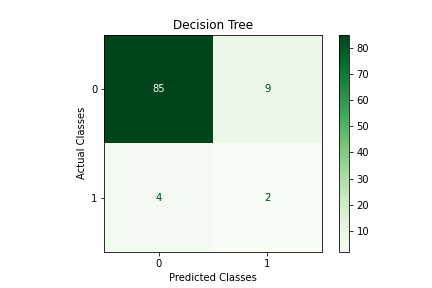
\includegraphics[width=1.2\textwidth]{CM1_DecisionTree_cm}
        \end{minipage}\hfill
        \begin{minipage}{0.25\textwidth}
            \centering
            \includegraphics[width=1.2\textwidth]{CM1_NaïveBayes_cm}
        \end{minipage}\hfill
        \begin{minipage}{0.25\textwidth}
            \centering
            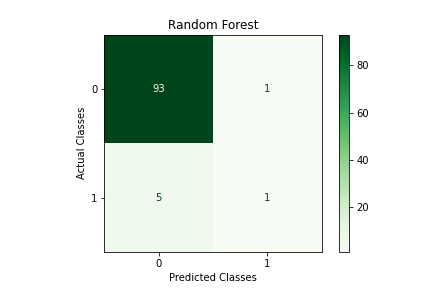
\includegraphics[width=1.2\textwidth]{CM1_RandomForest_cm}
        \end{minipage}\hfill
        \begin{minipage}{0.25\textwidth}
            \centering
            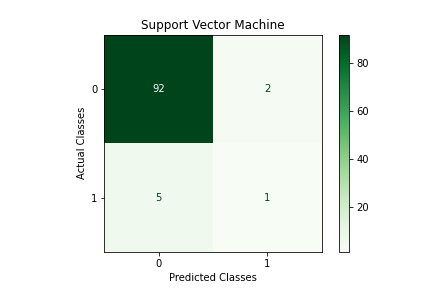
\includegraphics[width=1.2\textwidth]{CM1_SupportVectorMachine_cm}
        \end{minipage}\hfill
        \caption{Matriz de Confusão - Conjunto de dados CM1}\label{fig:mc_cm1}
    \end{figure}

    \begin{figure}
        \centering
        \begin{minipage}{0.25\textwidth}
            \centering
            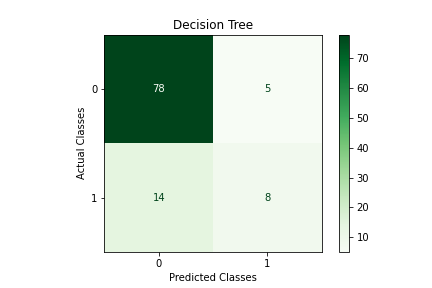
\includegraphics[width=1.2\textwidth]{KC2_DecisionTree_cm}
        \end{minipage}\hfill
        \begin{minipage}{0.25\textwidth}
            \centering
            \includegraphics[width=1.2\textwidth]{KC2_NaïveBayes_cm}
        \end{minipage}\hfill
        \begin{minipage}{0.25\textwidth}
            \centering
            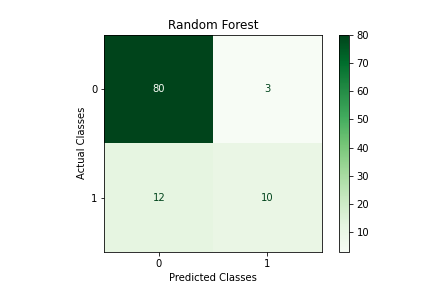
\includegraphics[width=1.2\textwidth]{KC2_RandomForest_cm}
        \end{minipage}\hfill
        \begin{minipage}{0.25\textwidth}
            \centering
            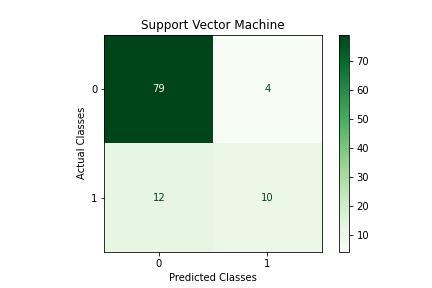
\includegraphics[width=1.2\textwidth]{KC2_SupportVectorMachine_cm}
        \end{minipage}\hfill
        \caption{Matriz de Confusão - Conjunto de dados KC2}\label{fig:mc_kc2}
    \end{figure}

    \begin{figure}
        \centering
        \begin{minipage}{0.25\textwidth}
            \centering
            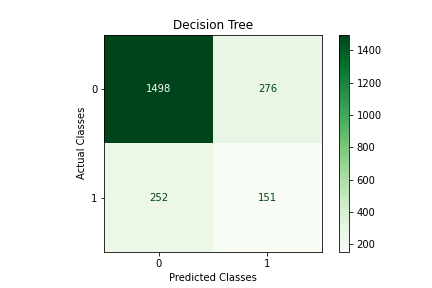
\includegraphics[width=1.2\textwidth]{JM1_DecisionTree_cm}
        \end{minipage}\hfill
        \begin{minipage}{0.25\textwidth}
            \centering
            \includegraphics[width=1.2\textwidth]{JM1_NaïveBayes_cm}
        \end{minipage}\hfill
        \begin{minipage}{0.25\textwidth}
            \centering
            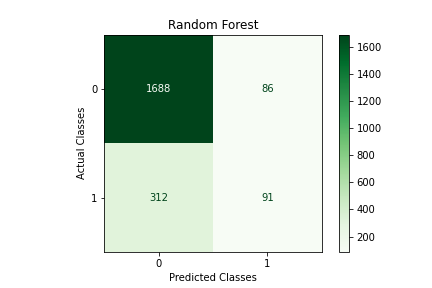
\includegraphics[width=1.2\textwidth]{JM1_RandomForest_cm}
        \end{minipage}\hfill
        \begin{minipage}{0.25\textwidth}
            \hspace{\fill}
        \end{minipage}\hfill
        \caption{Matriz de Confusão - Conjunto de dados JM1}\label{fig:mc_jm1}
    \end{figure}

    Não aplicamos a análise pelo algorítimo \textit{Support Vector Machine} ao conjunto de dados \textbf{JM1} por conta do tempo que seria necessário para executá-lo (ver Figuras \ref{fig:et_cm1}, \ref{fig:et_kc2} e \ref{fig:et_jm1}). Pela análise da Matriz de Confusão, o resultado consolidado de cada conjunto de dados, \textit{Support Vector Machine} não foi o método mais eficiente tampouco (ver Tabelas \ref{tab:mc_cm1}, \ref{tab:mc_kc2} e \ref{tab:mc_jm1}). Nas Tabelas \ref{tab:acc_cm1}, \ref{tab:acc_kc2} e \ref{tab:acc_jm1} podemos observar a acurácia dos algorítimos para cada classe - \textit{defects} - possui erros ($0 = \textit{não}, 1 = \textit{sim}$).

    \begin{table}[!ht]
        \renewcommand{\arraystretch}{1.2}
        \centering
        \scriptsize
        \begin{tabular}{ p{20mm} >{\raggedleft\arraybackslash}p{25mm} >{\raggedleft\arraybackslash}p{25mm} >{\raggedleft\arraybackslash}p{25mm} >{\raggedleft\arraybackslash}p{25mm} }
            \specialrule{.1em}{.05em}{.05em}
                Algorítimo & MCC:0 & MCC:1 & ACC:0 & ACC:1 \\
            \hhline{= = = = =}
                Random Forest &  0.2646763180494774 &  0.2646763180494774 &  0.94 &  0.94 \\
                SVM &  0.2024080616510014 &  0.2024080616510014 &  0.93 &  0.93 \\
                Naïve Bayes &  0.16585877695229945 &  0.16585877695229945 &  0.86 &  0.86 \\
                Decision Tree &  0.18033245722931218 &  0.18033245722931218 &  0.87 &  0.87 \\
            \specialrule{.1em}{.05em}{.05em}
        \end{tabular}
        \caption{Acurácia - Conjunto de dados CM1}\label{tab:acc_cm1}
    \end{table}

    \begin{table}[!ht]
        \renewcommand{\arraystretch}{1.2}
        \centering
        \begin{tabular}{ >{\raggedleft\arraybackslash}p{10mm} p{50mm} >{\raggedleft\arraybackslash}p{30mm} >{\raggedleft\arraybackslash}p{30mm} }
            \specialrule{.1em}{.05em}{.05em}
                Rank & Algorítimo & Pont. Classe & Pont. Geral \\
            \hhline{= = = =}
                1 & Random Forest & 6.05 & 2.18333 \\
                2 & Support Vector Machine & 5.55 & 1.81667 \\
                3 & Naïve Bayes & 4.95 & 1.65 \\
                3 & Decision Tree & 4.95 & 1.65 \\
            \specialrule{.1em}{.05em}{.05em}
        \end{tabular}
        \caption{Pontuação por análise da Matriz de Confusão - Conjunto de dados CM1}\label{tab:mc_cm1}
    \end{table}

    \begin{table}[!ht]
        \renewcommand{\arraystretch}{1.2}
        \centering
        \scriptsize
        \begin{tabular}{ p{20mm} >{\raggedleft\arraybackslash}p{25mm} >{\raggedleft\arraybackslash}p{25mm} >{\raggedleft\arraybackslash}p{25mm} >{\raggedleft\arraybackslash}p{25mm} }
            \specialrule{.1em}{.05em}{.05em}
                Algorítimo & MCC:0 & MCC:1 & ACC:0 & ACC:1 \\
            \hhline{= = = = =}
                Random Forest &  0.5169843329698582 &  0.5169843329698582 &  0.8571428571428571 &  0.8571428571428571 \\
                SVM &  0.48648427262381366 &  0.48648427262381366 &  0.8476190476190476 &  0.8476190476190476 \\
                Naïve Bayes &  0.3587866402333297 &  0.3587866402333297 &  0.819047619047619 &  0.819047619047619 \\
                Decision Tree &  0.3748813095095569 &  0.3748813095095569 &  0.819047619047619 &  0.819047619047619 \\
            \specialrule{.1em}{.05em}{.05em}
        \end{tabular}
        \caption{Acurácia - Conjunto de dados KC2}\label{tab:acc_kc2}
    \end{table}

    \begin{table}[!ht]
        \renewcommand{\arraystretch}{1.2}
        \centering
        \begin{tabular}{ >{\raggedleft\arraybackslash}p{10mm} p{50mm} >{\raggedleft\arraybackslash}p{30mm} >{\raggedleft\arraybackslash}p{30mm} }
            \specialrule{.1em}{.05em}{.05em}
                Rank & Algorítimo & Pont. Classe & Pont. Geral \\
            \hhline{= = = =}
                1 & Random Forest & 7.65 & 3.7 \\
                2 & Support Vector Machine & 6.75 & 3.5 \\
                3 & Naïve Bayes & 6.35 & 2.38333 \\
                3 & Decision Tree & 6.35 & 2.38333 \\
            \specialrule{.1em}{.05em}{.05em}
        \end{tabular}
        \caption{Pontuação por análise da Matriz de Confusão - Conjunto de dados KC2}\label{tab:mc_kc2}
    \end{table}

    \begin{table}[!ht]
        \renewcommand{\arraystretch}{1.2}
        \centering
        \scriptsize
        \begin{tabular}{ p{20mm} >{\raggedleft\arraybackslash}p{25mm} >{\raggedleft\arraybackslash}p{25mm} >{\raggedleft\arraybackslash}p{25mm} >{\raggedleft\arraybackslash}p{25mm} }
            \specialrule{.1em}{.05em}{.05em}
                Algorítimo & MCC:0 & MCC:1 & ACC:0 & ACC:1 \\
            \hhline{= = = = =}
                Naïve Bayes &  0.2102455048246325 &  0.2102455048246325 &  0.8203950390445567 &  0.8203950390445567 \\
                Decision Tree &  0.2143171951455535 &  0.2143171951455535 &  0.7574644005512172 &  0.7574644005512172 \\
                Random Forest &  0.2520032159505995 &  0.2520032159505995 &  0.8171796049609554 &  0.8171796049609554 \\
            \specialrule{.1em}{.05em}{.05em}
        \end{tabular}
        \caption{Acurácia - Conjunto de dados JM1}\label{tab:acc_jm1}
    \end{table}

    \begin{table}[!ht]
        \renewcommand{\arraystretch}{1.2}
        \centering
        \begin{tabular}{ >{\raggedleft\arraybackslash}p{10mm} p{50mm} >{\raggedleft\arraybackslash}p{30mm} >{\raggedleft\arraybackslash}p{30mm} }
            \specialrule{.1em}{.05em}{.05em}
                Rank & Algorítimo & Pont. Classe & Pont. Geral \\
            \hhline{= = = =}
                1 & Naïve Bayes & 5.05 & 1.81667 \\
                2 & Decision Tree & 4.95 & 2.18333 \\
                3 & Random Forest & 4.55 & 2.18333 \\
            \specialrule{.1em}{.05em}{.05em}
        \end{tabular}
        \caption{Pontuação por análise da Matriz de Confusão - Conjunto de dados JM1}\label{tab:mc_jm1}
    \end{table}

    Tendo em vista a grande diferença no tempo de execução para cada tipo de algorítimo, a opção de se utilizar \textit{Support Vector Machine} foi desconsiderada em nossa recomendação de solução para praticantes da indústria. A acurácia dos algorítimos é relativamente semelhante, o que também não é favorável para \textit{Support Vector Machine}, e \textit{Random Forest} mostrou-se ligeiramente superior para os conjuntos de dados menores. Já \textit{Naïve Bayes} mostrou-se mais eficiente aplicado ao conjunto de dados \textbf{JM1} com um número maior de instâncias.

    \begin{figure}
        \centering
        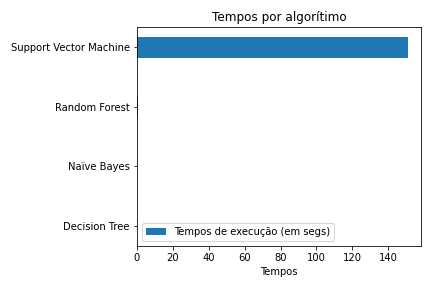
\includegraphics[width=0.9\textwidth]{CM1_elapsed_times}
        \caption{Tempos de execução para o conjunto de dados CM1}\label{fig:et_cm1}
    \end{figure}

    \begin{figure}
        \centering
        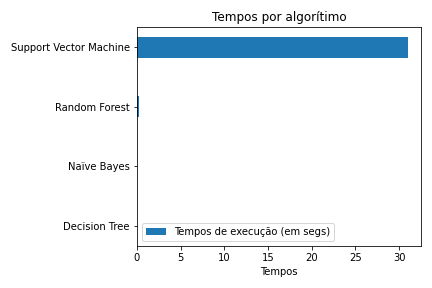
\includegraphics[width=0.9\textwidth]{KC2_elapsed_times}
        \caption{Tempos de execução para o conjunto de dados KC21}\label{fig:et_kc2}
    \end{figure}

    \begin{figure}
        \centering
        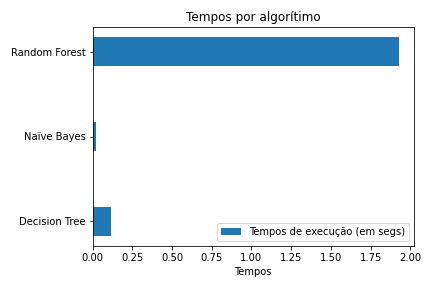
\includegraphics[width=0.9\textwidth]{JM1_elapsed_times}
        \caption{Tempos de execução para o conjunto de dados JM1}\label{fig:et_jm1}
    \end{figure}

\section{Trabalhos Relacionados}

    Diferentes técnicas tem sido aplicadas para prever falhas em ``\textit{software}'' \cite{abaei_empirical_2015,abdi_hybrid_2015,chatterjee_bayesian_2018,dhanalaxmi_adaptive_2015,diwaker_prediction_2018,felix_predicting_2020,gao_effective_2017,harikarthik_optimal_2019,jayanthi_software_2019,kalsoom_dimensionality_2018,kumaresan_software_2019,mahajan_design_2015,panda_slice-based_2016,rani_neural_2018,roya_neuro-genetic_2015,vitiello_software_2019}. Enquanto alguns autores preferem técnicas de aprendizado de máquina supervisionada \cite{rani_neural_2018} ou semi-supervisionada \cite{abaei_empirical_2015}, a maioria investiga uma abordagem híbrida utilizando conjuntamente métodos de busca evolutivos \cite{abdi_hybrid_2015,anwar_hybrid-adaptive_2019,dhanalaxmi_adaptive_2015,diwaker_prediction_2018,roya_neuro-genetic_2015,shamshiriRandomEvolutionarySearch2018,sharifipourStructuralTestData2018,tianTestDataGeneration2016,varshneyHybridParticleSwarm2018,yaoConstrainedMultiobjectiveTest2015}.


\section{Conclusão e Trabalhos Futuros}

    Neste estudo, a baixa acurácia obtida pelos métodos listados nos leva a crer que abordagens que aplicam \textit{ensembles} e as híbridas com métodos de busca sejam o próximo passo lógico a seguir. Apesar disto acreditamos que esta é uma solução simples, rápida e fácil de ser aplicada pelos praticantes, e se evitarmos utilizar \textit{Support Vector Machine} que exigirá uma alocação de tempo e recursos maiores, pode ser uma opção para inserir este tipo de análise num processo de desenvolvimento de \textit{software}.

    Além das abordagens utilizando \textit{ensembles} e em conjunto com métodos de busca, o próximo passo óbvio deste trabalho é aplicá-lo na priorização dos módulos que devem ser submetidos a testes mais rigorosos, tornando assim esta uma solução interessante para incrementar a qualidade e ao mesmo tempo reduzir os custos e os prazos de confecção e execução de testes.

    E finalmente, outra oportunidade que se mostra em aberto, é a possibilidade de utilizarmos as métricas de McCabe\cite{mccabe1976complexity} disponíveis no conjuntos de dados utilizados e que foram negligenciadas por este estudo.

\printnoidxglossary[type=acronym]
\printnoidxglossary[type=main]

\section{Referencias}

    \bibliographystyle{sbc}
    \begingroup
        \renewcommand{\section}[2]{}%
        \bibliography{JMG-BND}
    \endgroup

\end{document}